\documentclass[10pt]{beamer}

\usepackage[english]{babel}
\usepackage[utf8]{inputenc}
\usepackage[T1]{fontenc}
\usepackage{lmodern}

\usepackage{layout}
%\usepackage{epsfig}
\usepackage{graphicx}
\graphicspath{{../report/images/}}
\usepackage[outdir=../report/images/]{epstopdf}
\usepackage{subfigure}


\usepackage{siunitx}
\usepackage{eurosym}

\usepackage{amsthm}
\usepackage{amsmath}
\usepackage{amssymb}

\usepackage{mathrsfs}
\usepackage{wrapfig}
\usepackage{url}
\usepackage{multirow}
\usepackage{array}
\usepackage{pgfplots}

\usepackage[version=3]{mhchem}

\usepackage{wasysym}
%Bibtex
%\usepackage[square]{natbib}
%\newcommand{\newblock}{}

\usetheme{Warsaw}
\setbeamertemplate{headline}{}

\usepackage{graphicx}
\usepackage{epsfig}
\usepackage{epstopdf}

\usepackage{todonotes}
\title{Bank queue optimization}
\author[Malian DR, Florentin G, Quentin L, Harlod T]{
  \small
  Malian De Ron
  \and
  Florentin Goyens
  \\
  Quentin Laurent
  \and
  Harold Taeter
}

\begin{document}

\begin{frame}
  \maketitle
\end{frame}

\begin{frame}
  \frametitle{Model}
  \begin{block}{$M/G/2$ model}
  \begin{itemize}
    \item Arrivals of client follows a Poisson process
    \item 2 tellers
    \end{itemize}
  \end{block}
\end{frame}

  \begin{frame}
  \frametitle{Parameters estimation}
 
 \begin{itemize}
 \item Time varying rate of arrival $\lambda$ for the Poisson process. 
 \item $\lambda$ is assumed piecewise constant, 6 values over one day.  
\item Approximation: 
\[\frac{1}{\lambda}\approx \frac{ \text{Time elapsed} }{ \text{number of clients served}}\]  
 \end{itemize}  
  \end{frame}
  
  \begin{frame}
	\frametitle{Parameters estimation}

\begin{figure}
\centering
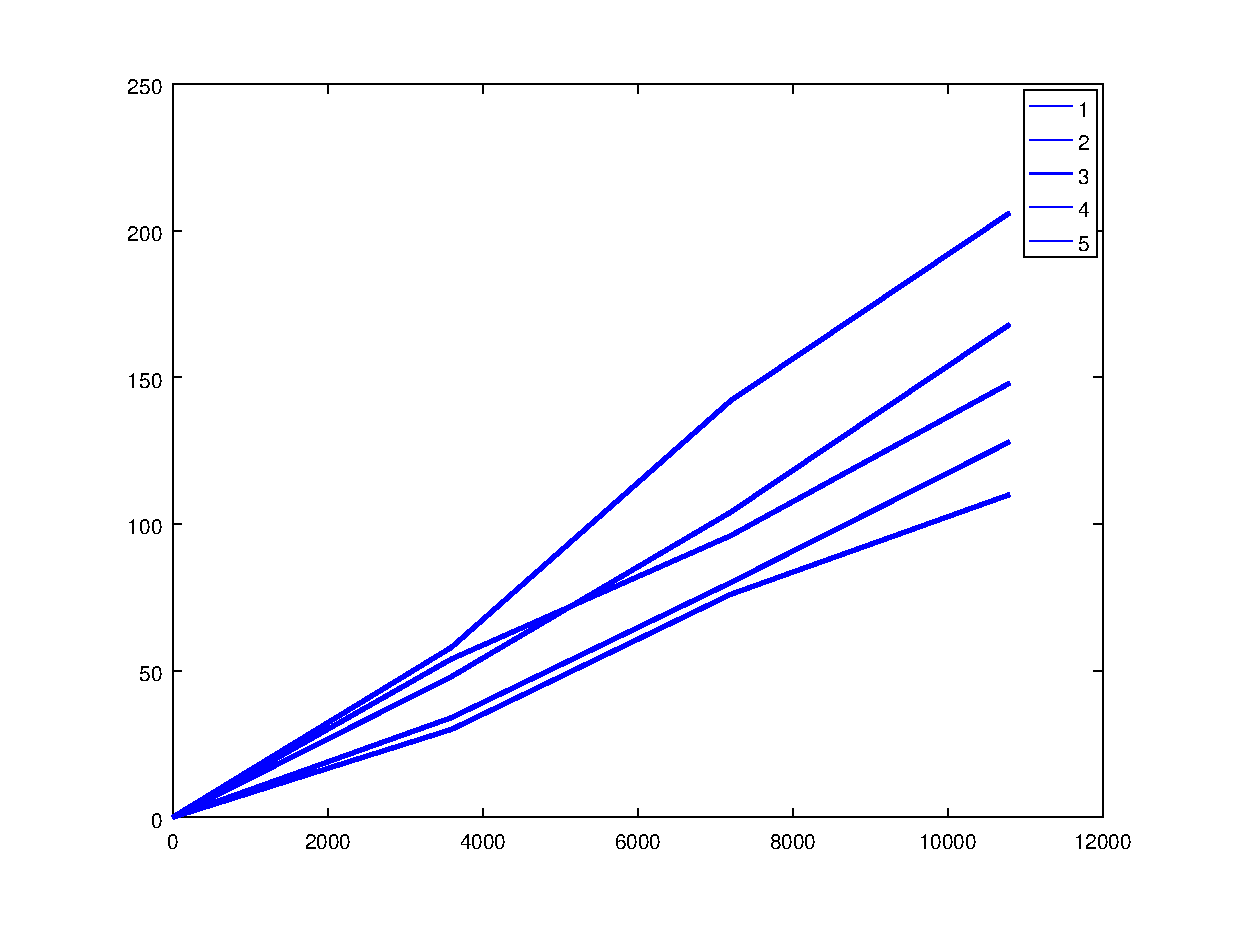
\includegraphics[width = \textwidth]{../report/images/lambdaApprox.eps}
\caption{Piecewise linear approximation of clients arrivals}
\end{figure}

\end{frame}

\begin{frame}
  \frametitle{Parameters estimation }
 
 \begin{itemize} 
  \item Service time at a desk 
  follows a lognormal distibution.
  \item Mean $=213.7[s]$ and standart deviation $=194.6[s]$ 
 \end{itemize} 
\begin{figure}[!h]
  \centering
  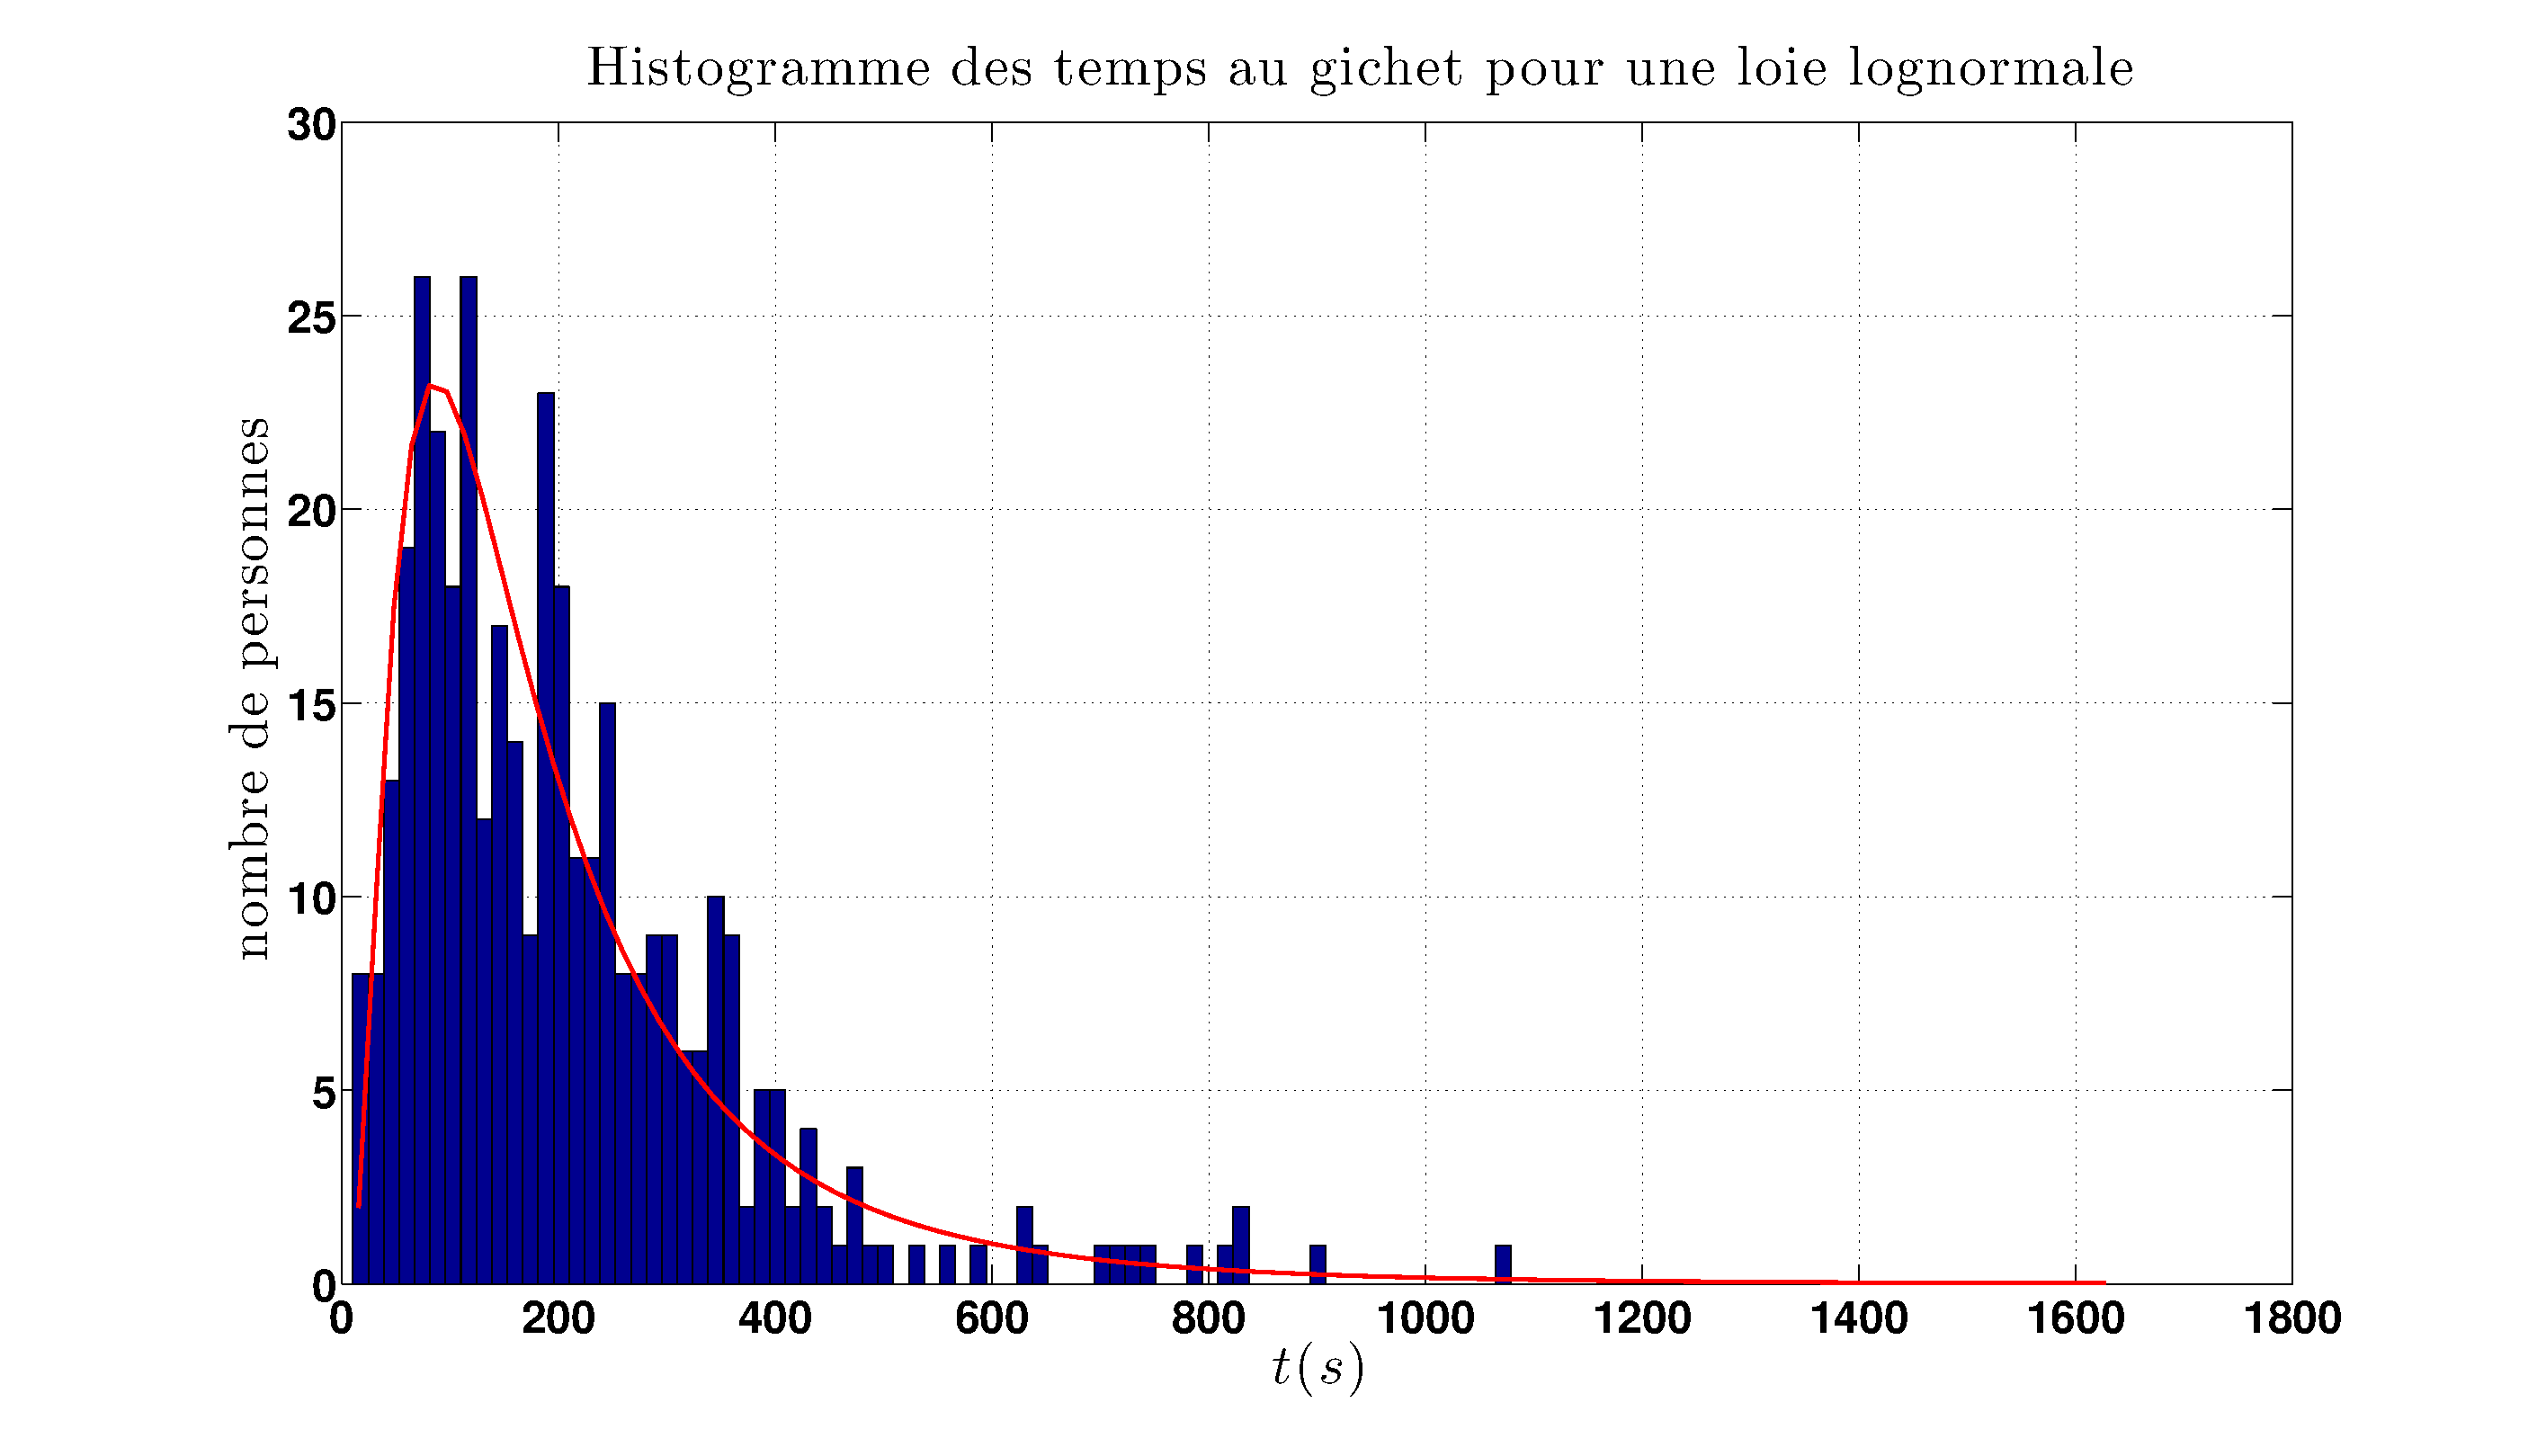
\includegraphics[width = 0.9\textwidth]{./hist_lognormal.eps}
  \end{figure}  
  
  
  
\end{frame}


\begin{frame}
  \frametitle{Anylogic model : non-merged}
  \begin{figure}
  \centering
\subfigure[Waiting time]{
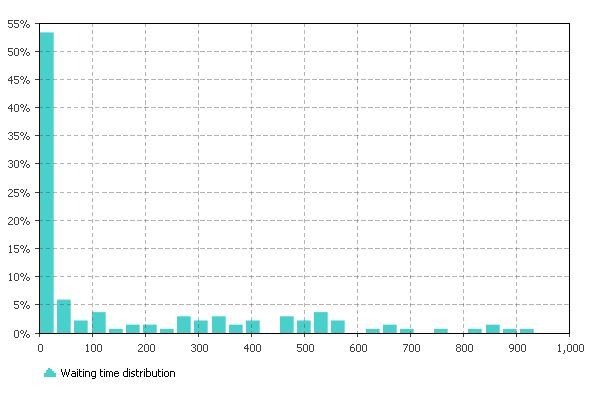
\includegraphics[width = 0.48\textwidth]{NM2telQ.jpg}
}
\subfigure[Total time in the system]{
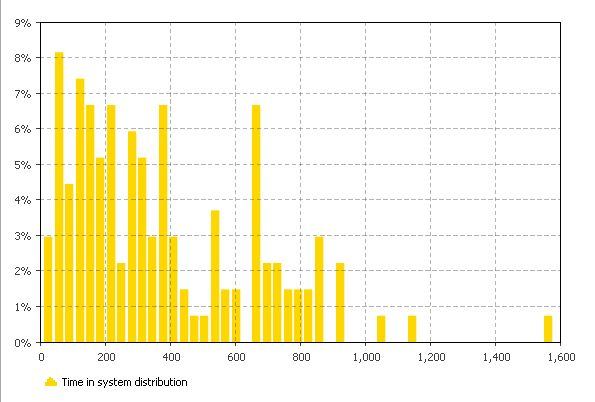
\includegraphics[width = 0.48\textwidth]{NM2telTOTAL.jpg}
}

\caption{Non-merged bank with 2 tellers}
  \end{figure}
  
\begin{table}
\centering
\begin{tabular}{|c|c|}
\hline
$\mu [min]$ & $t_{max} [min]$ \\
\hline
3 & 15 \\
\hline
\end{tabular} 
\end{table}

\end{frame}

\begin{frame}
  \frametitle{The merge project}
  \begin{block}{Modification of the model}
  \begin{itemize}
  \item  Clients arriving in the merged branches = sum of the two merged branches
  $\rightarrow $ new Poisson process with an arrival rate of the clients twice as big as that of the two old branches.
  \item Processing time follows the same distribution as before
  \end{itemize}
  \end{block}
 
\end{frame}

\begin{frame}
  \frametitle{Anylogic model II : Merged bank}
  \begin{figure}
  \centering
\subfigure[Waiting time]{
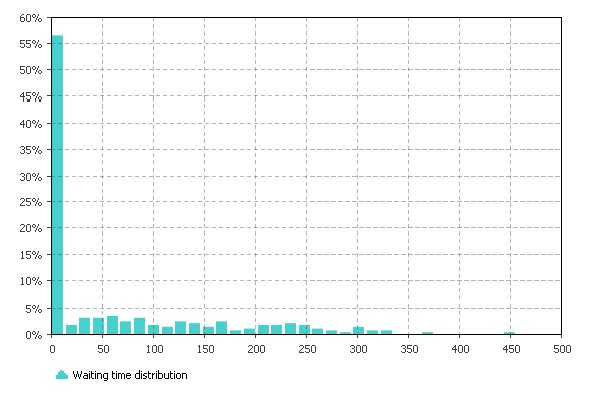
\includegraphics[width = 0.48\textwidth]{M4telQ.jpg}
}
\subfigure[Total time in the system]{
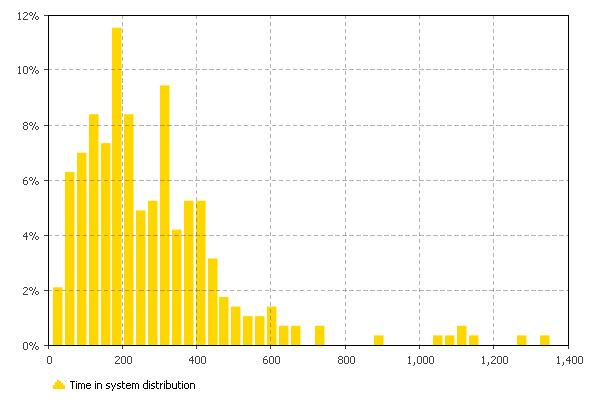
\includegraphics[width = 0.48\textwidth]{M4telTOTAL.jpg}
}

\caption{Merged bank with 4 tellers}
\end{figure}
  
  
\begin{table}
\centering
\begin{tabular}{|c|c|}
\hline
$\mu[min]$ & $t_{max}[min]$ \\
\hline
1 & 7 \\
\hline
\end{tabular} 
\end{table}

\end{frame}


\begin{frame}
  \frametitle{Anylogic model III : Merged bank}
\begin{figure}
\centering
\subfigure[Waiting time]{
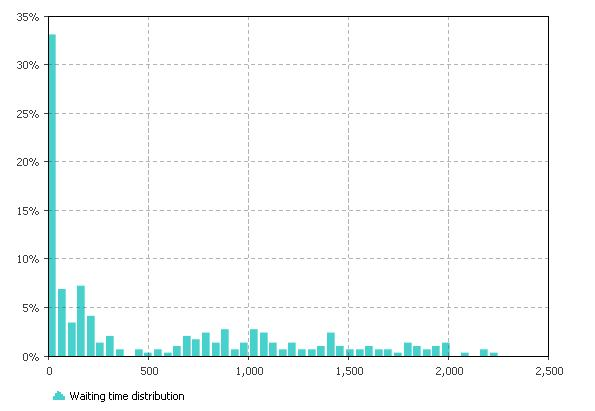
\includegraphics[width = 0.48\textwidth]{M3telQ.jpg}
}
\subfigure[Total time in the system]{
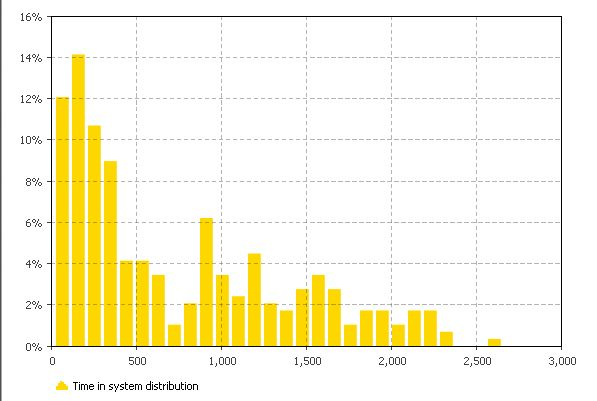
\includegraphics[width = 0.48\textwidth]{M3telTOTAL.jpg}
}
\caption{Merged bank with 3 tellers}
\end{figure}

\begin{table}
\centering
\begin{tabular}{|c|c|}
\hline
$\mu[min]$ & $t_{max}[min]$ \\
\hline
9 & 37 \\
\hline
\end{tabular} 
\end{table}

\end{frame}


\begin{frame}
  \frametitle{Anylogic model IV : Merged bank}
  \begin{figure}
  \centering
\subfigure[Waiting time]{
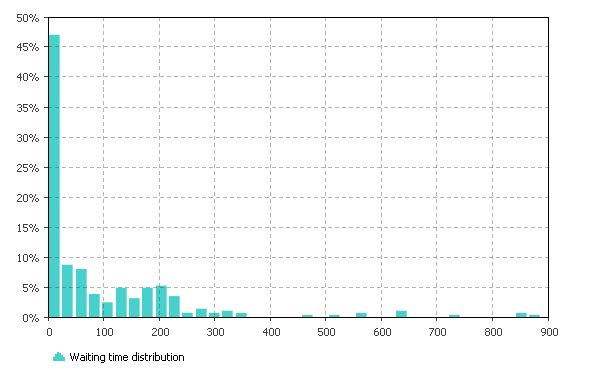
\includegraphics[width = 0.48\textwidth]{M3-4telQ.jpg}
}
\subfigure[Total time in the system]{
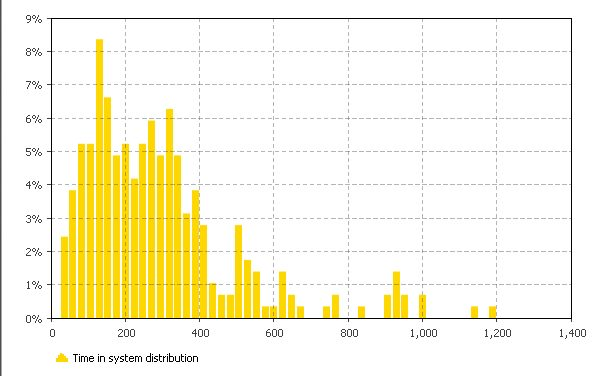
\includegraphics[width = 0.48\textwidth]{M3-4telTOTAL.jpg}
}

\caption{Merged bank with 3tellers in the morning and 4 tellers in the afternoon}
\end{figure}
  
  
\begin{table}
\centering
\begin{tabular}{|c|c|}
\hline
$\mu[min]$ & $t_{max}[min]$ \\
\hline
1.5 & 15 \\
\hline
\end{tabular} 
\end{table}

\end{frame}







\begin{frame}
\frametitle{Fluid approximation}
\begin{block}{Deterministic model}
\begin{itemize}
\item Instead of discrete arrivals, continuous arrivals with a rate $\lambda(t)$
\item $A(t) = \int_0^t \lambda(t)$ is the cumulative number of arrivals
\item $\omega (t) \leq c = N_t \cdot \frac{1}{\mu}$ is the departure rate of the queue, where $c$ is the maximum rate, $N_t$ the number of tellers and $\mu$ the mean processing time of a customer by a teller.
\item $S(t) = \int_0^t \omega(t)$ is the cumulative number of departures from the queue.
\end{itemize}
\end{block}
\begin{figure}
\centering
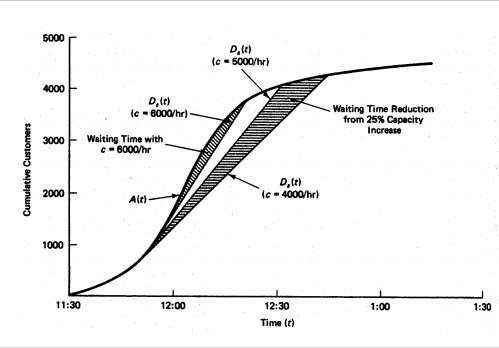
\includegraphics[width = 6cm]{fluid_approx.png}
\end{figure}
\end{frame}

\begin{frame}
\frametitle{Optimum number of servers}
\begin{block}{What is our cost?}
\begin{itemize}
\item Proportional to the capacity we can handle and the waiting time of the clients
\begin{eqnarray*}
\min_c & & \alpha c + \beta \int_D A(t)-S(t)\\
\end{eqnarray*}
where $D = \{t | A(t)>=S(t) \}$
\item The number of tellers must be an integer $\rightarrow$ additional constraint : $N_t = c \cdot \mu$ must be integer
\end{itemize}
\end{block}
\begin{figure}
\centering
\begin{tabular}{|c|c|c|c|}
\hline 
1/2 day salary(\euro ) & Half day time(s) & $\alpha$(\euro $s$/clients) & $\beta$(\euro/clients$\cdot s$) \\ 
 \hline 
$75$ & $10800$ & $0.433526$ & $3.47222e-07$ \\ 
 \hline 
 
 \end{tabular}
\end{figure}
\end{frame}

\begin{frame}
\frametitle{Results : who gets fired?}
\begin{figure}
\centering
\subfigure[Monday pm]{
\includegraphics[width = 0.48\textwidth]{half\string_daylundi\string_pm\string_clients\string_served.eps}
}
\subfigure[Friday am]{
\includegraphics[width = 0.48\textwidth]{half\string_dayvendredi\string_am\string_clients\string_served.eps}
}

\caption{Cumulative number of client served.}
\end{figure}
\begin{center}
$N_t = $ $ 3 $
\end{center}
\end{frame}
\end{document}
